\subsection{Patterns}
Des patterns ? Ah ouais ? Ah non des patrons. Quoi ? Des motifs ? Des schémas ?
Décidément, l'anglais technique c'est pas très clair ! Ici il va falloir
reconnaitre des \sout{patrons} motifs et appuyer sur les bons boutons.
\begin{modulebox}{Pas terne}
  \begin{hangingpar}
    \begin{flushright}
    \textit{\dots Il fallait que je la fasse celle là}
    \end{flushright}
  \end{hangingpar}
  \modulesection{Description}
  \begin{moduleaction}[Difficulté]
    Pas si facile quand même
  \end{moduleaction}
  \hline%
  \modulesection{Composants :}
  \begin{moduleaction}[boutons]
    Il faut appuyer dessus pour valider un choix. Attention à ne pas se tromper.
  \end{moduleaction}
  \begin{moduleaction}[écran Arduino TFT]
    Un écran LCD rétroéclairé muni d'un emplacement pour carte SD. Avec ça, on
    peut générer tout un tas de formes géométriques et même charger des images.
  \end{moduleaction}
\end{modulebox}
\begin{dndtable}
	\textbf{Difficulté} & \textbf{Image correcte} \\
	Facile & \qquad
\includegraphics[height=1cm]{img/vim.jpg} \\
	Moyen & \qquad
\includegraphics[height=1cm]{img/cat.jpg} \\
	Difficile & \qquad
\includegraphics[height=1cm]{img/logo.jpg} \\
\end{dndtable}

\noindent Et si vous avez un doute dites-vous que c'est l'heure du jugement dernier\ldots
\newline
\vspace{0.5cm}
\centerline{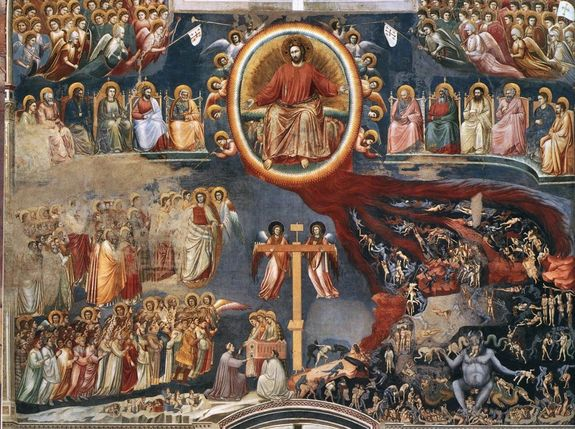
\includegraphics[height=4cm]{img/jugement-dernier.jpg}}
\newpage
